\documentclass[conference]{IEEEtran}
\IEEEoverridecommandlockouts
\usepackage[utf8]{inputenc}
\usepackage[T1]{fontenc}
\usepackage[brazil]{babel}
\usepackage{cite}
\usepackage{amsmath,amssymb,amsfonts}
\usepackage{algorithmic}
\usepackage{graphicx}
\usepackage{textcomp}
\usepackage{xcolor}
\usepackage{booktabs}
\def\BibTeX{{\rm B\kern-.05em{\sc i\kern-.025em b}\kern-.08em
    T\kern-.1667em\lower.7ex\hbox{E}\kern-.125emX}}
\begin{document}

\title{Embeddings de not\'icias financeiras e comunicados do Copom em portugu\^es na previs\~ao do retorno di\'ario do Ibovespa\\\large Entrega preliminar: solu\c{c}\~ao proposta e replica\c{c}\~ao de baselines}

\author{\IEEEauthorblockN{Hiago Lacerda}
\IEEEauthorblockA{\textit{Deep Learning} \\
\textit{Universidade Federal de Pernambuco - UFPE}\\
Recife, Brasil \\
hwal@cin.ufpe.br}
}

\maketitle

\begin{abstract}
Este documento reporta o est\'agio inicial de um trabalho que investiga se embeddings textuais de not\'icias financeiras e o sinal de pol\'itica monet\'aria do Copom, em portugu\^es, melhoram a previs\~ao do retorno di\'ario (D+1) do Ibovespa. Descrevem-se a solu\c{c}\~ao proposta e o protocolo de valida\c{c}\~ao adotado, e reportam-se os experimentos j\'a conclu\'idos nesta etapa: a replica\c{c}\~ao de quatro baselines financeiros (passeio aleat\'orio, ARIMA, ARIMAX e XGBoost) sob valida\c{c}\~ao walk-forward. A integra\c{c}\~ao de embeddings textuais (BERTimbau, FinBERT-PT-BR) e do sinal do Copom encontra-se em desenvolvimento e n\~ao \'e reportada aqui.
\end{abstract}

\begin{IEEEkeywords}
previs\~ao de s\'eries financeiras, embeddings de texto, BERTimbau, FinBERT, valida\c{c}\~ao walk-forward, Ibovespa
\end{IEEEkeywords}

\section{Solu\c{c}\~ao Proposta}
\label{sec:solucao}

O trabalho investiga se fontes textuais em portugu\^es -- not\'icias de jornais financeiros e comunicados de pol\'itica monet\'aria do Copom -- possuem poder preditivo sobre o retorno di\'ario (D+1) do Ibovespa, quando avaliadas sob um protocolo que exclui explicitamente qualquer forma de vazamento temporal de informa\c{c}\~ao. A motiva\c{c}\~ao segue a literatura de combina\c{c}\~ao de LSTM com embeddings financeiros \cite{gu2024finbertlstm} e de compara\c{c}\~ao de modelos de sentimento em finan\c{c}as \cite{dahal2023comparative}, que reportam ganhos preditivos modestos e sens\'iveis ao protocolo de valida\c{c}\~ao empregado, e na disponibilidade de modelos de linguagem especializados em finan\c{c}as em portugu\^es \cite{araci2019finbert}.

A solu\c{c}\~ao proposta consiste numa progress\~ao incremental de complexidade, na qual cada n\'ivel serve de refer\^encia ao seguinte: (1) passeio aleat\'orio e ARIMA/ARIMAX, como pisos cl\'assicos de compara\c{c}\~ao; (2) XGBoost treinado exclusivamente com vari\'aveis de pre\c{c}o, como baseline tabular n\~ao-recorrente; (3) uma rede LSTM parcimoniosa treinada apenas com pre\c{c}o; e (4) a mesma LSTM acrescida, separadamente, de embeddings textuais de manchetes do InfoMoney (via BERTimbau e FinBERT-PT-BR) e do sinal de pol\'itica monet\'aria do Copom (classificado por zero-shot em vi\'es \emph{hawkish}/\emph{dovish}). Um ganho real de texto ou de Copom deve manifestar-se como melhora mensur\'avel sobre o n\'ivel (3), e n\~ao apenas em compara\c{c}\~ao com os pisos cl\'assicos. Fontes adicionais consideradas na proposta original -- Valor Econ\^omico e redes sociais (X/Twitter) -- foram deixadas fora do escopo desta etapa, em favor de aprofundar a compara\c{c}\~ao entre as duas fontes prim\'arias (InfoMoney e Copom) sob rigor estat\'istico maior.

A valida\c{c}\~ao adota esquema walk-forward expans\'ivel (nunca parti\c{c}\~ao aleat\'oria), com embargo temporal entre treino e teste, e toda transforma\c{c}\~ao dependente dos dados -- normaliza\c{c}\~ao, redu\c{c}\~ao de dimensionalidade, calibra\c{c}\~ao, sele\c{c}\~ao de ordem do ARIMA -- ajustada exclusivamente no conjunto de treino de cada partic\~ao (fold). O alvo \'e o log-retorno de D+1,
\begin{equation}
y_t = \ln\!\left(\frac{\text{close}_{t+1}}{\text{close}_t}\right),
\label{eq:target}
\end{equation}
avaliado por magnitude do erro (MAE, RMSE), acerto direcional (\emph{directional accuracy}, MCC) e signific\^ancia estat\'istica formal: habilidade direcional por Pesaran-Timmermann \cite{pesaran1992}, e compara\c{c}\~oes pareadas entre modelos por Diebold-Mariano \cite{diebold1995} (com corre\c{c}\~ao de pequena amostra \cite{harvey1997}) na etapa final, ambos com corre\c{c}\~ao de Holm para m\'ultiplas compara\c{c}\~oes.

\section{Dados}

A s\'erie di\'aria do Ibovespa (\^{}BVSP), julho/2018--dezembro/2024, foi obtida junto ao Stooq e validada contra refer\^encias p\'ublicas conhecidas (fundo da crise da COVID-19 e fechamento de 2024, desvio de 0,00\% em ambos). O per\'iodo de estudo (janeiro/2019--dezembro/2024) totaliza 1.492 preg\~oes com alvo definido.

Manchetes do InfoMoney (se\c{c}\~oes \emph{mercados} e \emph{economia}) j\'a foram integralmente coletadas: 57.611 registros, cobrindo 100\% dos preg\~oes do per\'iodo de estudo (Fig.~\ref{fig:manchetes}), com atribui\c{c}\~ao temporal por corte \`as 17h (fechamento da B3), tratando corretamente o hor\'ario de ver\~ao hist\'orico. Os 49 comunicados do Copom (2018--2024) tamb\'em j\'a foram coletados via API de dados abertos do Banco Central. A extra\c{c}\~ao de embeddings e a integra\c{c}\~ao dessas fontes ao modelo LSTM constituem a pr\'oxima etapa do trabalho.

\begin{figure}[htbp]
\centerline{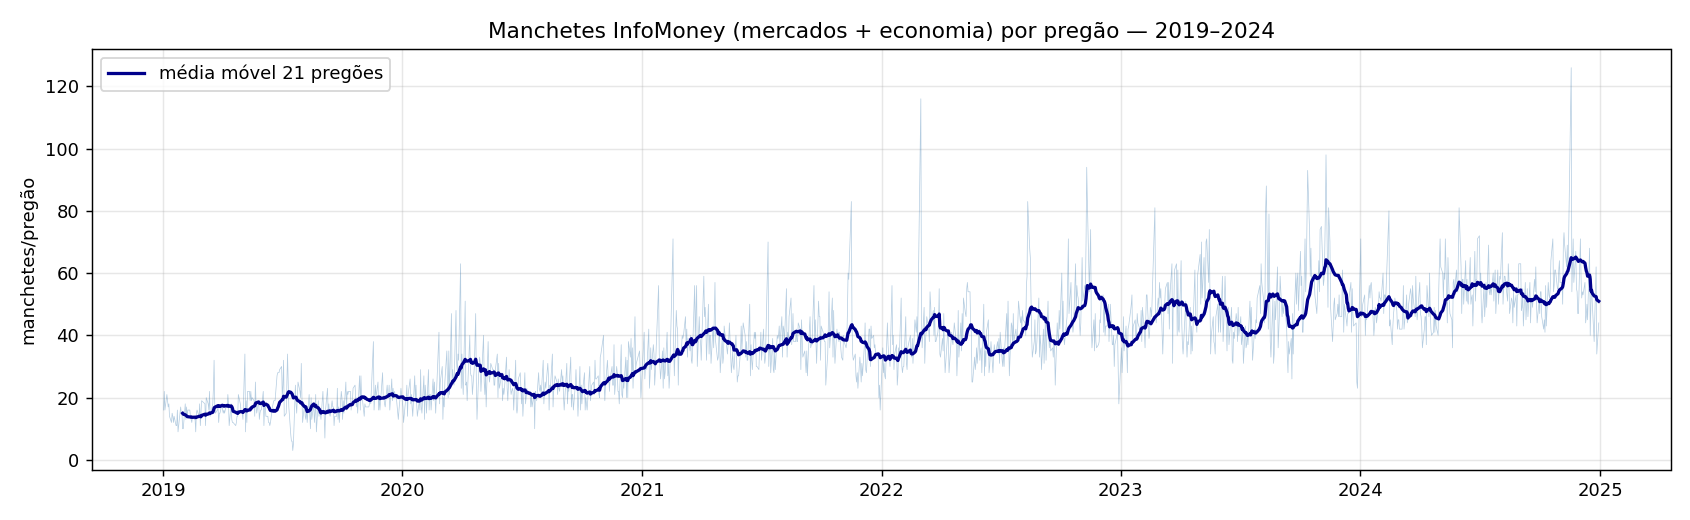
\includegraphics[width=0.48\textwidth]{manchetes_por_pregao.png}}
\caption{Manchetes coletadas por preg\~ao, 2019--2024.}
\label{fig:manchetes}
\end{figure}

\section{Experimentos: Replica\c{c}\~ao de Baselines}
\label{sec:baselines}

Esta etapa concentrou-se em estabelecer, com rigor, os patamares de compara\c{c}\~ao que qualquer modelo com texto precisar\'a superar -- priorizando a replica\c{c}\~ao correta dos baselines financeiros cl\'assicos antes da integra\c{c}\~ao de texto.

A Fig.~\ref{fig:acf} apresenta a autocorrela\c{c}\~ao do retorno di\'ario e do retorno ao quadrado, diagn\'ostico que fundamenta a sele\c{c}\~ao de ordem do ARIMA. O retorno exibe estrutura linear fraca (teste de estacionariedade ADF: estat\'istica $-11{,}86$, $p\approx7\times10^{-22}$, justificando $d=0$); o retorno ao quadrado exibe \emph{clustering} de volatilidade bem mais pronunciado, evid\^encia de que a previsibilidade dispon\'ivel na s\'erie concentra-se majoritariamente na vari\^ancia, n\~ao na dire\c{c}\~ao -- padr\~ao consistente com a hip\'otese de efici\^encia informacional de mercado.

\begin{figure}[htbp]
\centerline{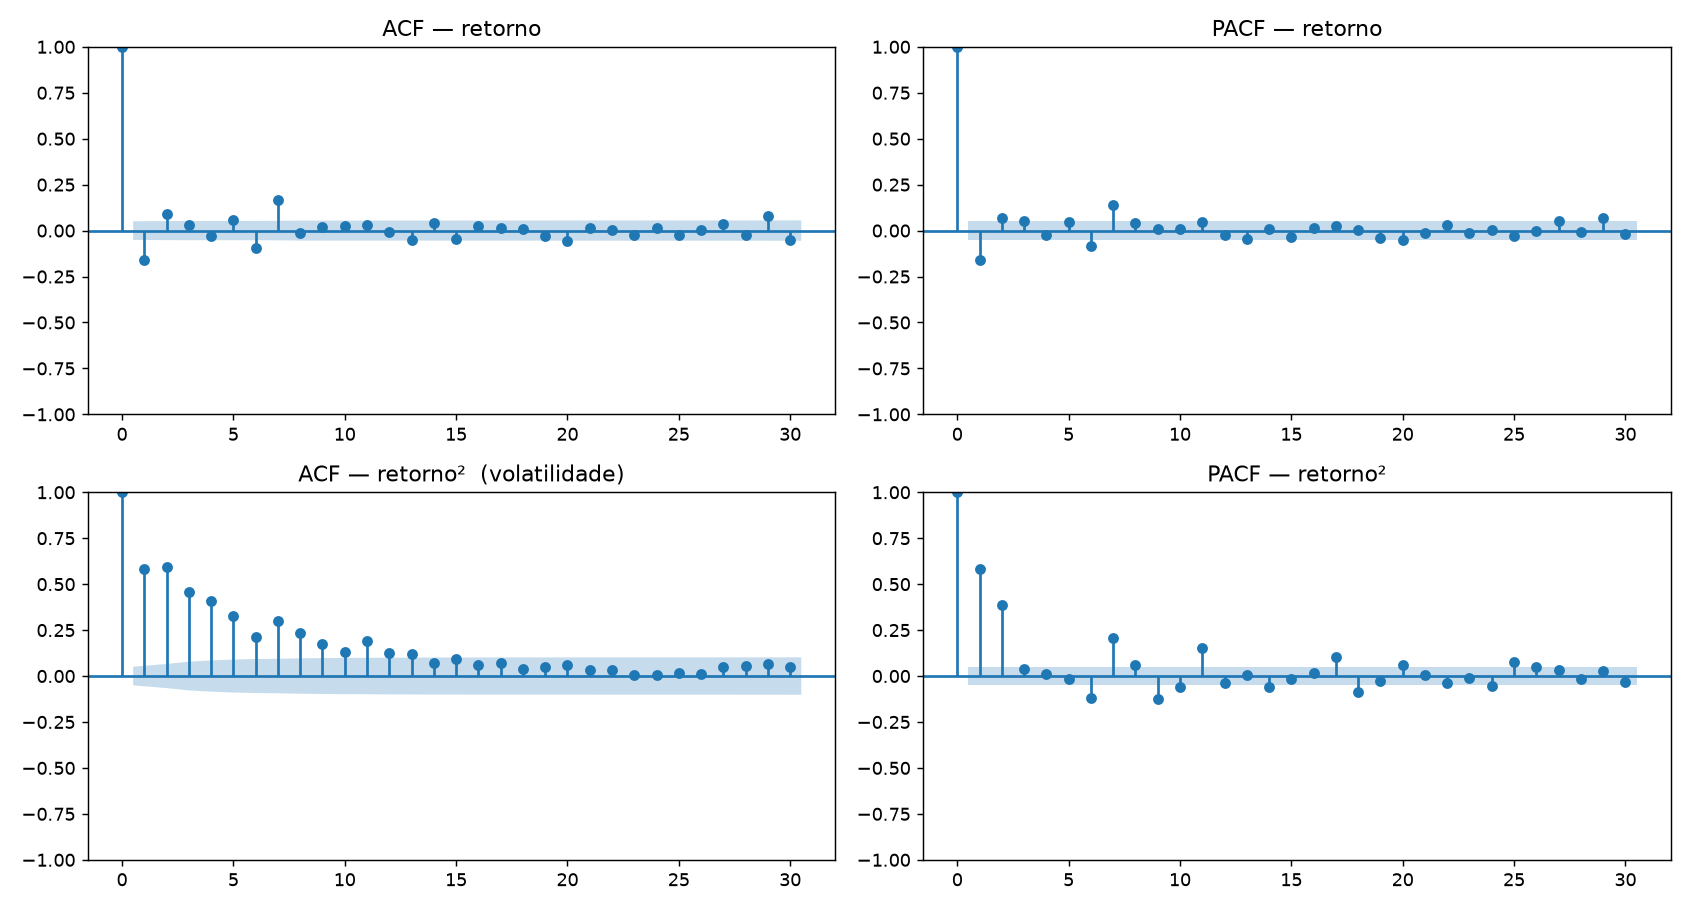
\includegraphics[width=0.48\textwidth]{acf_pacf_retorno.png}}
\caption{ACF/PACF do retorno di\'ario do Ibovespa.}
\label{fig:acf}
\end{figure}

Quatro baselines foram implementados e avaliados sob o mesmo protocolo walk-forward que ser\'a usado para os modelos com texto: passeio aleat\'orio (retorno previsto = 0, dire\c{c}\~ao por persist\^encia), ARIMA (ordem por AIC via \texttt{auto\_arima}, reajustado a cada fold), ARIMAX (com \texttt{n\_noticias} e dispers\~ao dos embeddings do dia como vari\'aveis ex\'ogenas padronizadas por fold) e XGBoost (treinado exclusivamente com as 18 vari\'aveis de pre\c{c}o, calibra\c{c}\~ao isot\^onica, $N$=10 sementes). A Tabela~\ref{tab:baselines} resume os resultados.

\begin{table}[htbp]
\caption{Baselines replicados (fonte: \texttt{tabela\_comparativa\_final.csv})}
\begin{center}
\begin{tabular}{lcccc}
\toprule
\textbf{Modelo} & \textbf{MAE} & \textbf{RMSE} & \textbf{DA} & \textbf{PT $p$ (Holm)} \\
\midrule
Random Walk & 0,0116 & 0,0159 & 0,485 & 1,000 \\
ARIMA       & 0,0120 & 0,0166 & 0,522 & 1,000 \\
ARIMAX      & 0,0124 & 0,0181 & 0,511 & 1,000 \\
XGBoost     & 0,0117 & 0,0161 & 0,515 & 0,577 \\
\bottomrule
\end{tabular}
\label{tab:baselines}
\end{center}
\end{table}

Nenhum dos quatro baselines atinge signific\^ancia direcional a 5\% pelo teste de Pesaran-Timmermann \cite{pesaran1992} ap\'os corre\c{c}\~ao de Holm; o XGBoost, o mais competitivo dos quatro, chega mais perto ($p=0{,}577$), mas permanece longe do limiar. O ARIMA supera marginalmente o passeio aleat\'orio em acur\'acia direcional (52,2\% vs.\ 48,5\%), consistente com a estrutura linear fraca identificada na Fig.~\ref{fig:acf}, mas essa vantagem n\~ao se traduz, ainda, em signific\^ancia estat\'istica formal. O volume de negocia\c{c}\~ao foi validado como sinal financeiramente plaus\'ivel antes de ser inclu\'ido como vari\'avel: correla\c{c}\~ao com retorno absoluto de +0,18, consistente com a literatura \cite{karpoff1987}, e persist\^encia estatisticamente significativa (Ljung-Box, $p\approx0$).

\section{Discuss\~ao}

A replica\c{c}\~ao dos baselines j\'a antecipa o principal desafio deste trabalho: a s\'erie de retornos di\'arios do Ibovespa exibe pouqu\'issima estrutura explor\'avel por modelos lineares simples -- nenhum dos quatro baselines testados supera o acaso de forma estatisticamente significativa --, o que estabelece uma barra alta e honesta para qualquer ganho atribu\'ido \`a inclus\~ao de texto. Isso \'e consistente com a hip\'otese de efici\^encia informacional de mercado, sob a qual informa\c{c}\~ao publicamente dispon\'ivel tende a ser rapidamente incorporada ao pre\c{c}o.

Essa mesma hip\'otese motiva a quest\~ao que orienta a pr\'oxima etapa do trabalho: mais relevante do que perguntar se o texto \emph{cont\'em} sinal sobre o mercado \'e perguntar \emph{quando} esse sinal se manifesta em rela\c{c}\~ao ao pre\c{c}o. \'E plaus\'ivel que not\'icias financeiras descrevam com fidelidade eventos j\'a conhecidos pelo mercado no momento da publica\c{c}\~ao -- e portanto j\'a precificados --, em vez de anteciparem eventos futuros. Essa quest\~ao ser\'a investigada diretamente na pr\'oxima etapa, comparando a correla\c{c}\~ao do sentimento textual extra\'ido pelo FinBERT-PT-BR com o retorno do \emph{mesmo} dia da not\'icia versus o retorno do dia seguinte (o alvo dos modelos) -- compara\c{c}\~ao que, independentemente do resultado, informar\'a diretamente a interpreta\c{c}\~ao dos ganhos (ou da aus\^encia deles) observados quando o texto for integrado \`a LSTM.

\begin{thebibliography}{00}
\bibitem{araci2019finbert} D. Araci, ``FinBERT: Financial Sentiment Analysis with Pre-trained Language Models,'' \emph{arXiv preprint arXiv:1908.10063}, 2019.
\bibitem{diebold1995} F. X. Diebold and R. S. Mariano, ``Comparing Predictive Accuracy,'' \emph{Journal of Business \& Economic Statistics}, vol. 13, no. 3, pp. 253--263, 1995.
\bibitem{harvey1997} D. Harvey, S. Leybourne, and P. Newbold, ``Testing the Equality of Prediction Mean Squared Errors,'' \emph{International Journal of Forecasting}, vol. 13, no. 2, pp. 281--291, 1997.
\bibitem{karpoff1987} J. M. Karpoff, ``The Relation Between Price Changes and Trading Volume: A Survey,'' \emph{Journal of Financial and Quantitative Analysis}, vol. 22, no. 1, pp. 109--126, 1987.
\bibitem{pesaran1992} M. H. Pesaran and A. Timmermann, ``A Simple Nonparametric Test of Predictive Performance,'' \emph{Journal of Business \& Economic Statistics}, vol. 10, no. 4, pp. 461--465, 1992.
\bibitem{gu2024finbertlstm} W. Gu, Y. Zhong, S. Li, C. Wei, L. Dong, Z. Wang, and C. Yan, ``Predicting Stock Prices with FinBERT-LSTM: Integrating News Sentiment Analysis,'' in \emph{Proc. 8th Int. Conf. on Cloud and Big Data Computing (ICCBDC)}, Oxford, UK, 2024. DOI: 10.1145/3694860.3694870.
\bibitem{dahal2023comparative} K. R. Dahal, N. R. Pokhrel, S. Gaire, S. Mahatara, R. P. Joshi, A. Gupta, H. R. Banjade, and J. Joshi, ``A comparative study on effect of news sentiment on stock price prediction with deep learning architecture,'' \emph{PLOS ONE}, vol. 18, no. 4, e0284695, 2023.
\end{thebibliography}

\end{document}
